\documentclass[border=2pt]{standalone}
\usepackage{tikz}
\usetikzlibrary{arrows.meta}
\begin{document}
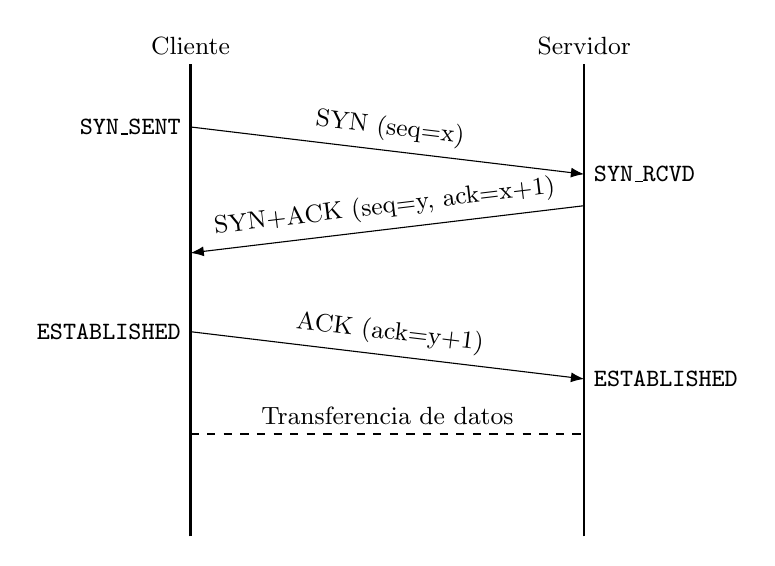
\begin{tikzpicture}[>=Latex, font=\small]
  \draw[thick] (0,0) -- (0,6);
  \draw[thick] (5,0) -- (5,6);
  \node[above] at (0,6) {Cliente};
  \node[above] at (5,6) {Servidor};

  \draw[->] (0,5.2) -- (5,4.6) node[midway, above, sloped] {SYN (seq=x)};
  \draw[<-] (0,3.6) -- (5,4.2) node[midway, above, sloped] {SYN+ACK (seq=y, ack=x+1)};
  \draw[->] (0,2.6) -- (5,2.0) node[midway, above, sloped] {ACK (ack=y+1)};

  \node[left] at (0,5.2) {\texttt{SYN\_SENT}};
  \node[right] at (5,4.6) {\texttt{SYN\_RCVD}};
  \node[left] at (0,2.6) {\texttt{ESTABLISHED}};
  \node[right] at (5,2.0) {\texttt{ESTABLISHED}};

  \draw[dashed] (0,1.3) -- (5,1.3) node[midway, above] {Transferencia de datos};
\end{tikzpicture}
\end{document}
